\chapter{Konzeption}
\label{sec_konzeption}

\section{Offlinefähigkeit}
\label{sec_konzeption_offline}

\subsection{Caching statischer Ressourcen}
\label{subsec_konzept_caching-statische-ressourcen}

Während Webanwendungen einen Fehler anzeigen, sobald der Benutzer ohne aktive Internetverbindung versucht zu einer Seite zu navigieren, ist es in nativen Apps möglich sich weiter innerhalb der Anwendung zu bewegen. 

Eine hybride Webanwendung muss also die Möglichkeit haben, zu erkennen, ob eine Internetverbindung vorhanden ist oder nicht und entsprechend reagieren. Hier kommt die Service Worker API ins Spiel. Hauptaugenmerkt der Technologie ist die Bereitstellung einer optimalen Offline"=Benutzererfahrung.   

Wie in \todo{Hier muss die Referenz hin} beschrieben handelt es sich beim Service Worker um eine Art Proxy zwischen der Webanwendung und dem Browser. Dadurch ist es möglich, Responses von HTTP-Request aufzunehmen und anzupassen. Dies ist eine Schlüsselfunktion, um Offlinefähigkeit anbieten zu können.

\begin{table}[h]
\centering
\begin{tabularx}{\textwidth}{| l | X | }
    \hline
    \textbf{Bezeichnung} & \textbf{Beschreibung} \\
    \hline
    networkOnly & Ressourcen werden nur aus Netzwerk geholt \\
    \hline    
    cacheOnly & Ressourcen werden immer aus Cache geladen \\
    \hline
    fastest & Versucht von beiden Quellen zu laden und Antwortet mit schnellerem Response \\
    \hline
    networkFirst & Versucht zuerst aus dem Netzwerk zu laden und schaut in den Cache, wenn dies fehlschlägt \\
    \hline
    cacheFirst & Bezieht Ressourcen direkt aus dem Cache, fragt jedoch auch beim Netzwerk nach und aktualisiert bei Erfolg die Ressourcen im Cache \\
    \hline
\end{tabularx}
\caption{Übersicht Caching Strategien}
\label{tbl_konzeption_caching-strategien}
\end{table}

Tabelle \ref{tbl_konzeption_caching-strategien} zeigt die fünf grundsätzlich möglichen Strategien für das Caching von statischen Ressourcen, die mit Hilfe des Service Workers umgesetzt werden können. Damit die Benutzung der Anwendung auch ohne aktive Internetverbindung gewährleistet ist, müssen die Ressourcen ebenfalls bereitstehen, wenn das Gerät offline ist. Dadurch das erkannt werden kann, ob das Gerät vom Internet getrennt ist und dadurch anders auf HTTP-Requests reqgieren werden kann, ergibt sich die Möglichkeit, Ressourcen auszuliefern, die lokal gespeichert sind.

Für den vorliegenden An \code{cacheFirst}-Verfahren bietet sich für die vorligenden Anwendungsfall an. Die angeforderten Ressourcen werden direkt aus dem Cache geladen und anschließend wird versucht, ob dieses mit Ressourcen aus dem Internet aktualisiert werden können(vgl. Bild \ref{image_konzept_caching-strategie}. Dadurch wird die Seite unabhängig vom Onlinezustand bei Anforderung schnell geladen.

\begin{figure}[htp] \centering{

\includegraphics[width=0.9\textwidth]{images/konzept_cache.pdf}}
\caption{Caching Strategie}
\label{image_konzept_caching-strategie}
\end{figure} 

\subsection{Caching des anwendungspezifischen Modells}
\label{subsec_konzeption_caching-modell}

Neben der in Abschnitt \ref{subsec_konzept_caching-statische-ressourcen} beschriebenen Vorhaltung der statischen Ressourcen muss die hybride Webanwendung ebenfalls einen Mechanismus zur Verfügung stellen, um das Datenmodell im Offlinebetrieb bereitzustellen.

\newpage
\section{Web Push}
\label{subsubsec_konzeption_serviceworker_push-api}

\begin{figure}[htp] \centering{
\centering
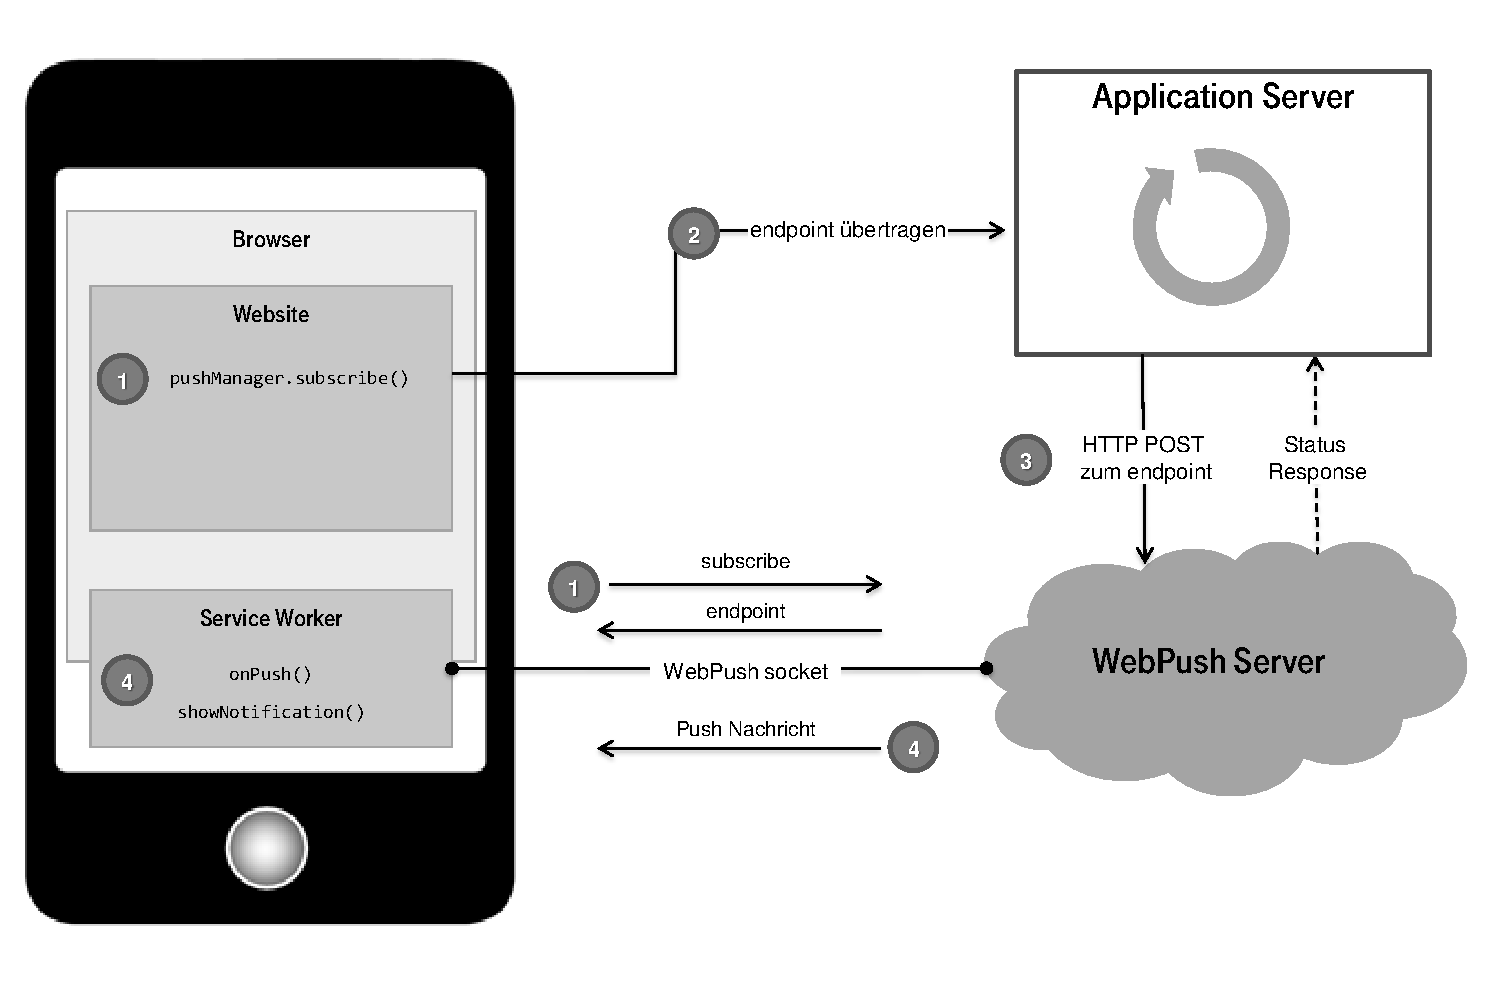
\includegraphics[width=0.9\textwidth]{images/architektur_serviceworker_push.pdf}}
\caption{Push mittels Serviceworker (in Anlehnung an MozillaWiki \cite{MOZ_WIKI})}
\quelle\url{https://wiki.mozilla.org/File:PushNotificationsHighLevel.png}
\label{image_architektur-serviceworker-push}
\end{figure}  


\todo{Beschreibung (mit Schema) der Softwarearchitektur ...}

\newpage
\section{Architekturbeschreibung}
\label{sec_konzeption_serviceworker_architektur}

Die Anwendung beruht auf dem Client-Server-Prinzip. Dabei stellt der Client lediglich die Oberfläche zur Interaktion mit dem Anwender dar. Außer der notwendigen UI- und Serviceworker-Logik ist die gesamte Geschäftslogik auf einen Business-Server (Applicationserver) ausgelagert. Die zentrale Datenbank sowie die statischen Ressourcen zur Darstellung des Client werden ebenfalls vom Applicationserver bereitgestellt. Für die Kommunikation steht eine RESTful-Schnittstelle zur Verfügung.

\begin{figure}[htp] \centering{
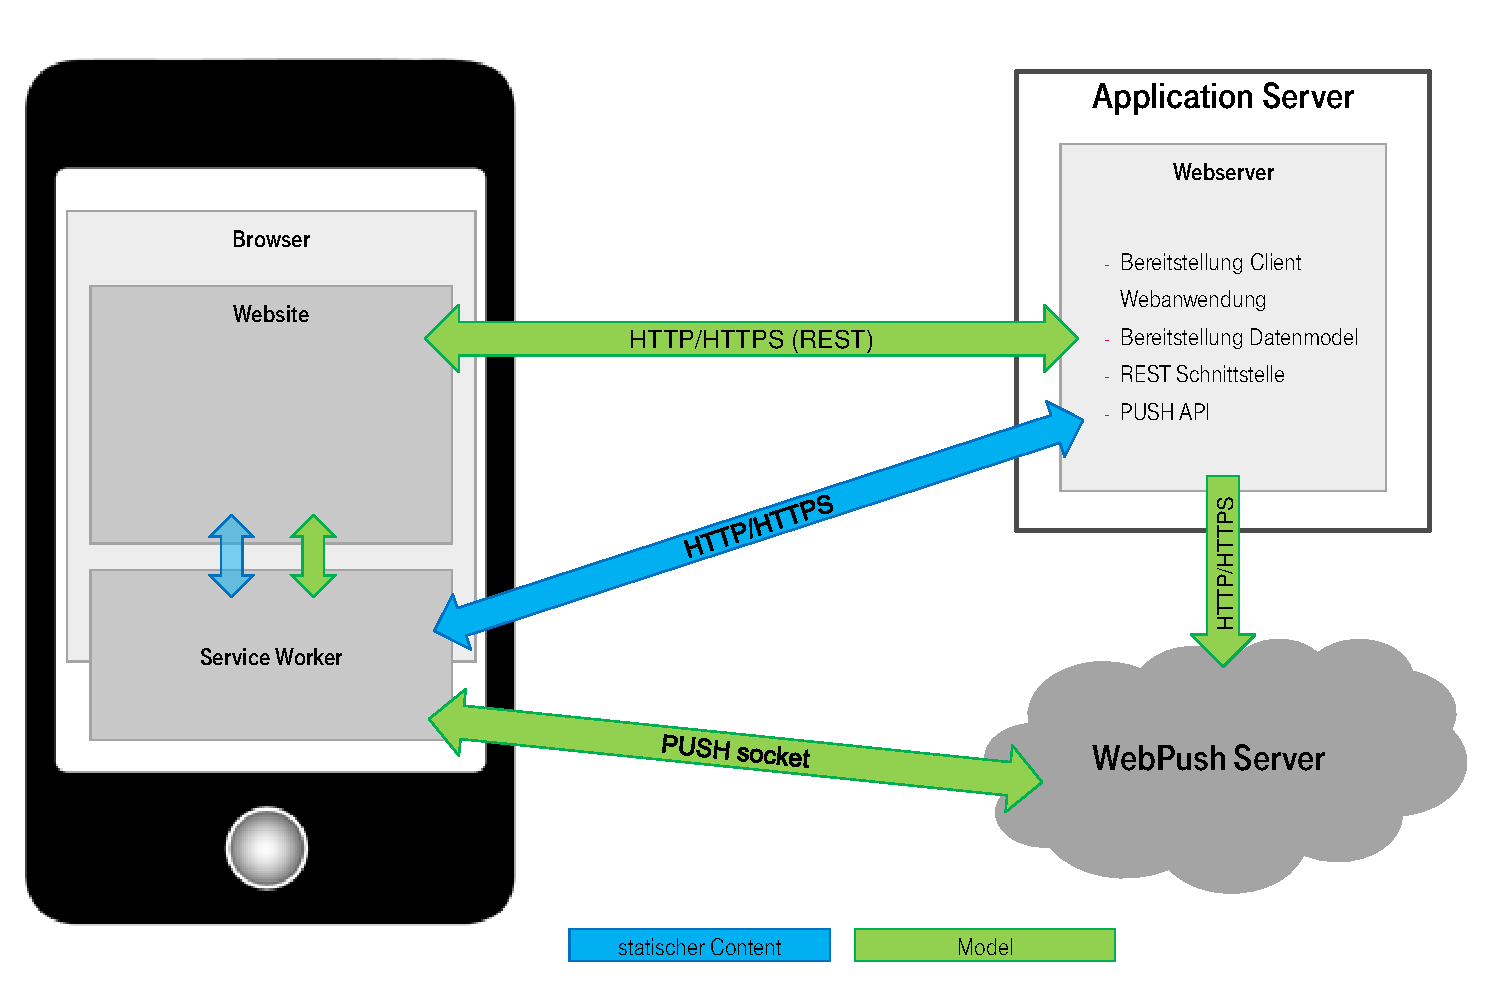
\includegraphics[width=0.9\textwidth]{images/architektur_serviceworker.pdf}}
\caption{Archtikturbeschreibung - Umsetzung mit Serviceworker}
\label{image_architektur-serviceworker-push}
\end{figure} 

\newpage
\section{Applicationserver}
\label{sec_konzeption_applicationserver}

\subsection{Datenbank}



\subsection{REST-API}

Zur Bereitstellung von CRUD-Funktionalitäten über standardisierte HTTP-Methoden (vgl. \ref{subsec_anforderungen_server} Anforderungen an Serverkomponente) wird dem Applicationserver eine RESTful-Schnittstelle hinzugefügt. Eine Übersicht über mögliche API-Routen mit entsprechender HTTP-Methode ist in Tabelle \ref{tbl_konzeption_rest} dargestellt. \\

\begin{table}[h]
\centering
\begin{tabular}{l | c | l }
    \textbf{Route} & \textbf{HTTP-Methode} & \textbf{Beschreibung} \\
    \hline\hline
    /api/signup & POST & Registriert einen neuen Benutzer \\
    /api/authenticate & POST & Authentifiziert einen Benutzer \\
    \hline
    /api/tasks & GET & Gibt alle Aufgaben zurück \\
    /api/tasks & POST & Legt eine neue Aufgabe an \\
    /api/tasks/:taskId & GET & Gibt eine einzelne Aufgabe zurück \\
    /api/tasks/:taskId & PUT & Aktualisiert eine einzelne Aufgabe \\
    /api/tasks/:taskId & DELETE & Löscht eine einzelne Aufgabe \\
    \hline
    /push/devices & GET & Gibt alle registrierten Geräte zurück \\
    /push/devices & POST & Registriert ein neues Gerät \\
\end{tabular}
\caption{Übersicht API Routen}
\label{tbl_konzeption_rest}
\end{table}

\subsubsection{Authentifizierung und Autorisierung} 

Für den Zugriff auf die CRUD-Methoden ist eine Benutzerauthentifizierung und Autorisierung notwendig. Dazu wird das Token-Verfahren verwendet.

\newpage
\section{Client-Oberfläche}
\label{sec_konzeption_client-ui}


... Mockup ... \\
... Beschreibung des UI ...\\

Um das \glqq{}Look and Feel\grqq{} einer nativen App zu erreichen wird das UI-Framework \textbf{nativeDroid2} verwendet. \\

\newpage
\section{Datenmodel}
\label{sec_konzeption_datamodel}

\begin{figure}[htp] \centering{
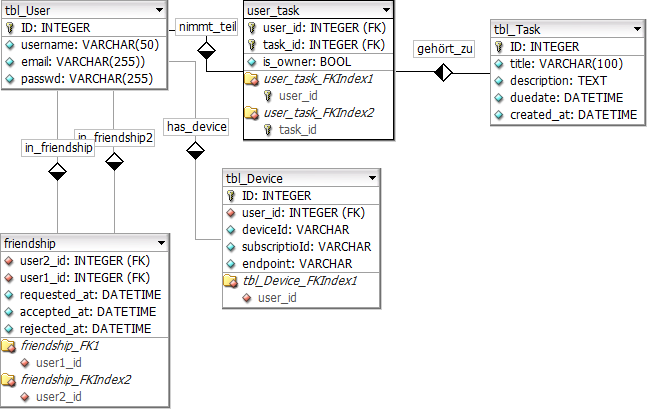
\includegraphics[width=0.9\textwidth]{images/model.png}}
\caption{Datenmodell}
\label{image_konzeption_datenmodell}
\end{figure} 
